%!TEX root=Principal.tex
\chapter{PROJETANDO TESTES EM INTERAÇÃO HUMANO-ROBÔ}
\label{cap:projetoihr}
Esse capítulo é dedicado a toda fase de preparação para os testes e estudos em Interação Humano-Robô~(IHR). É apresentado um conjunto de variáveis e como foram selecionadas para o teste de objetivo específico na interação. Quais são os fatores de projetos que devem ser considerados, preparação do robô e do ambiente, definição do contexto de uso. A execução do experimento e como é coletada cada informação sobre a IHR. Análise dos primeiros resultados obtidos para criação de um mecanismo probabílistico que auxilie na classificação do usuário. Todos esses pontos estão ilustrados na figura~\ref{fig:experimento}.

\begin{figure}[ht!]
	\centering
	\begin{minipage}{\textwidth}
		\caption{Visão geral sobre o projeto de IHR desenvolvido.}
		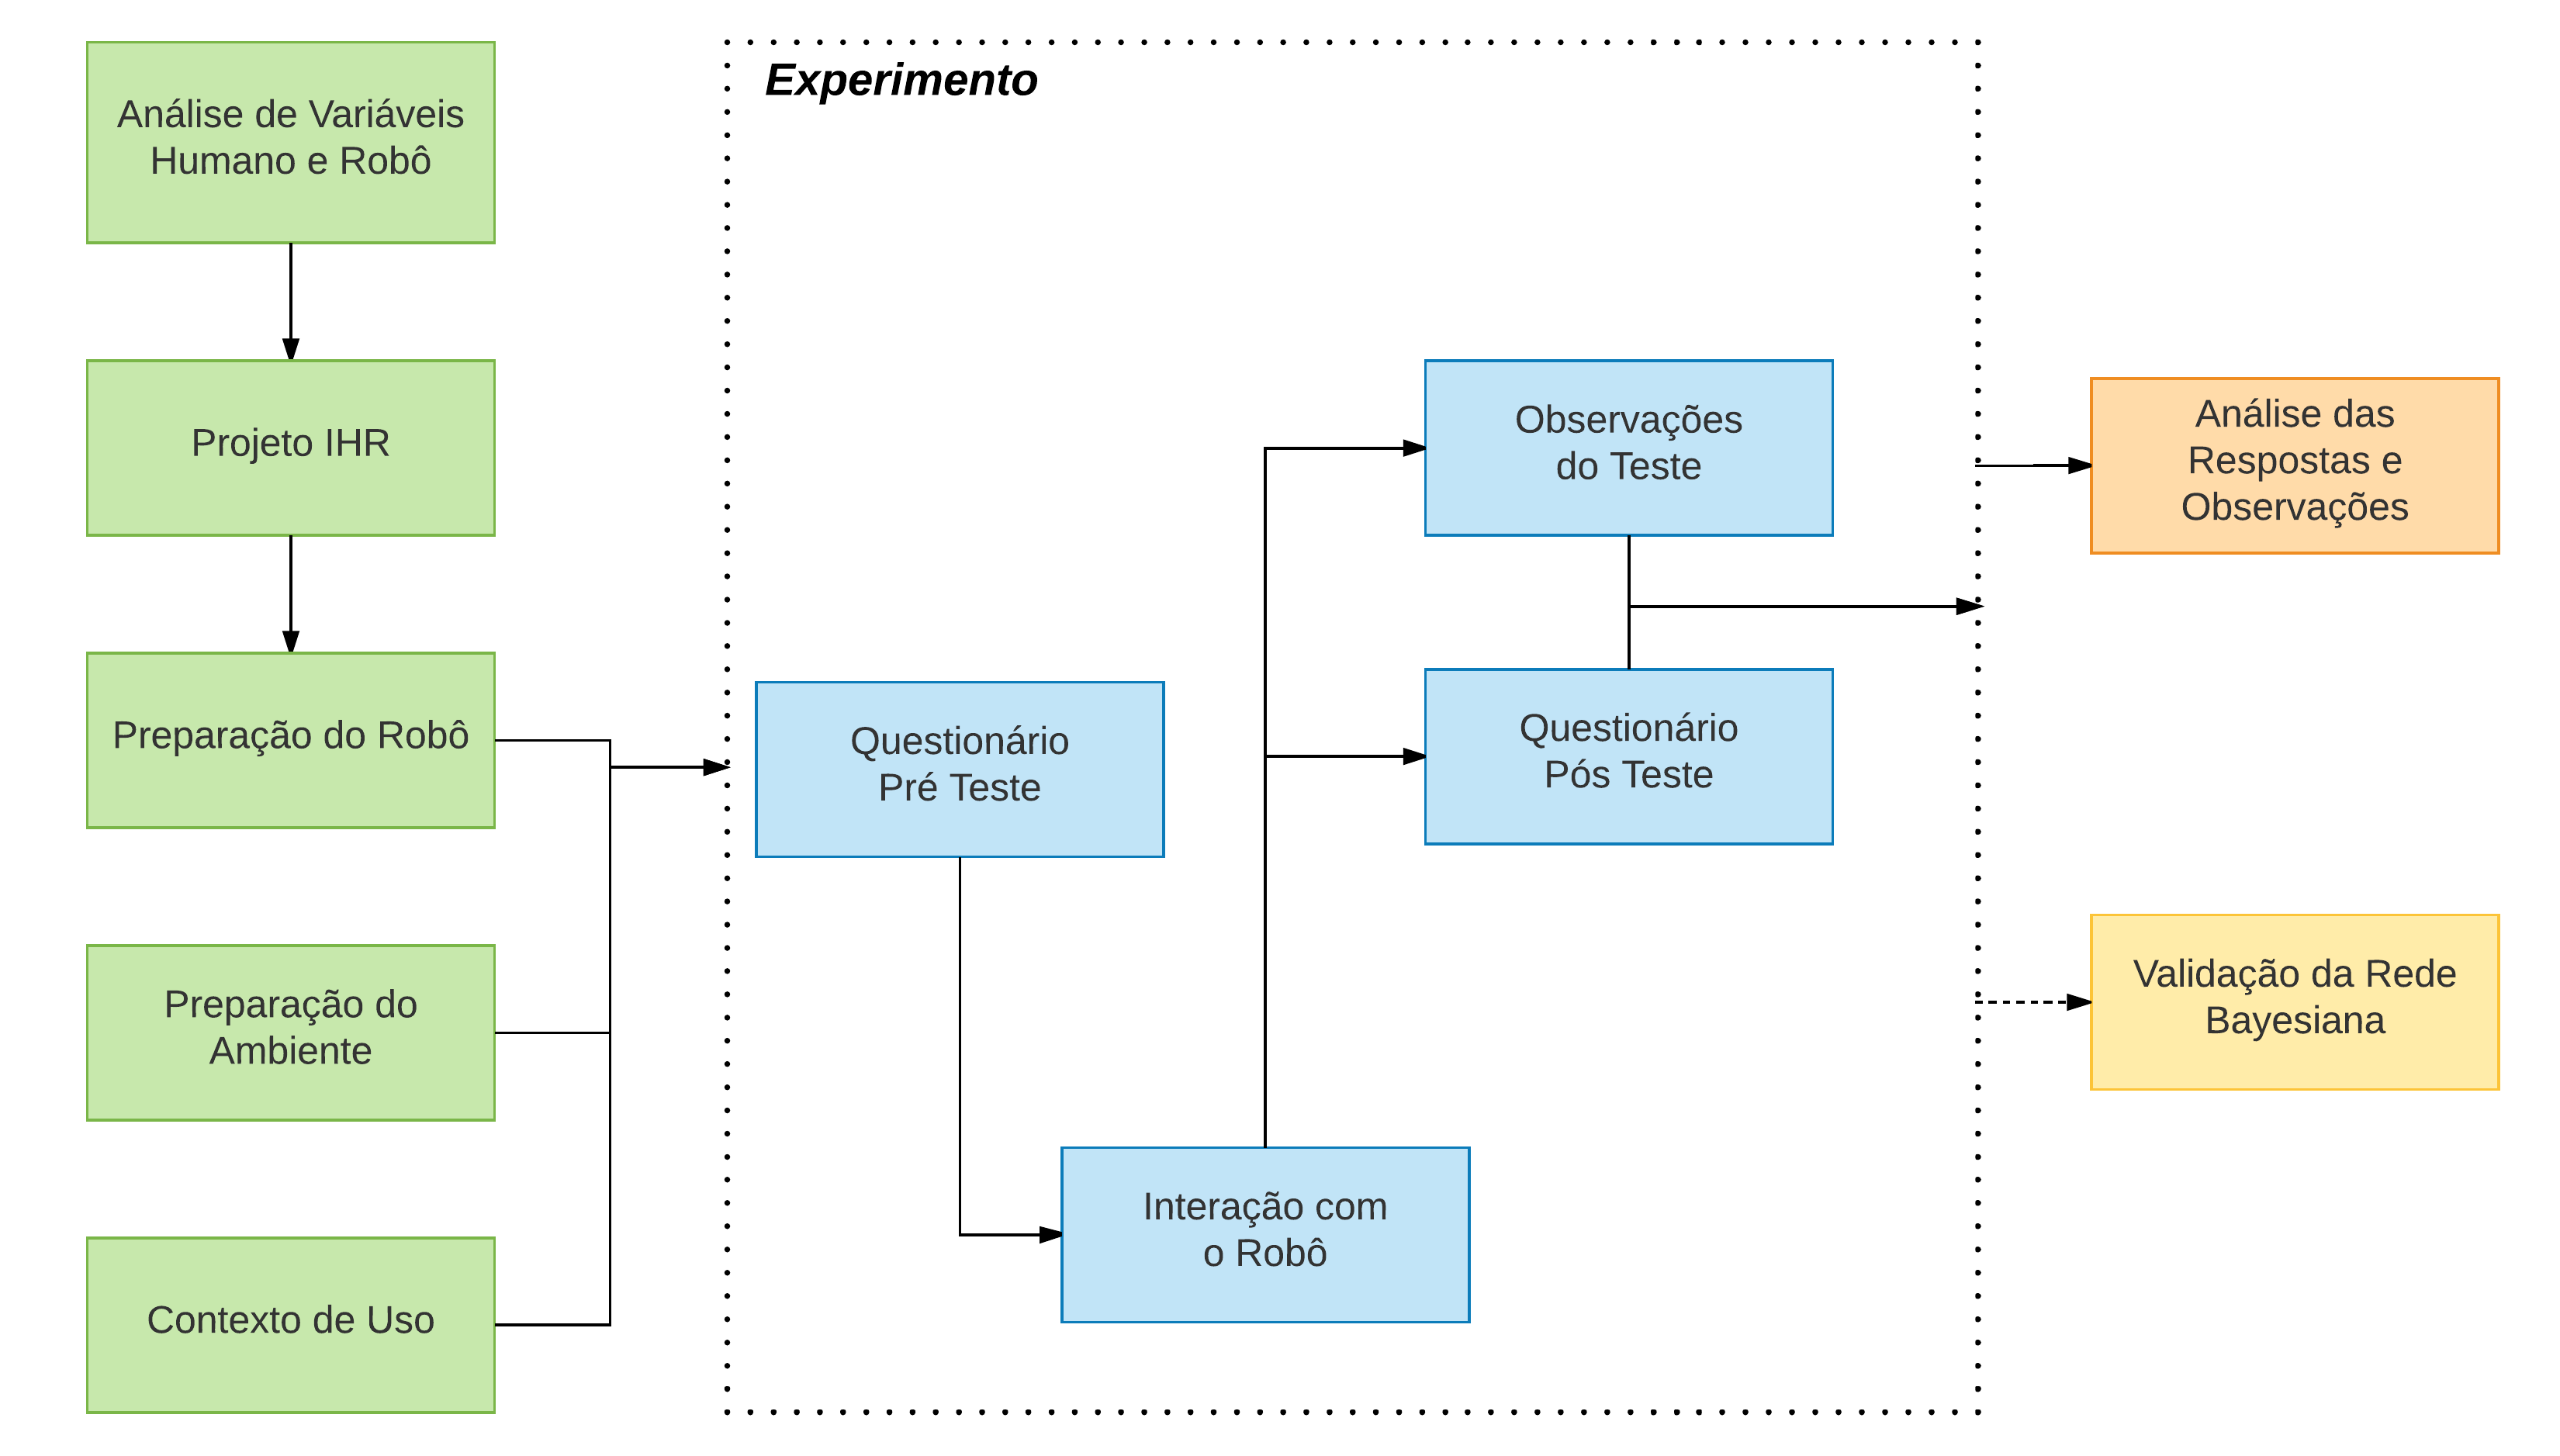
\includegraphics[width=\textwidth]{experimento.png}
		\smallcaption{Fonte: o autor.}
		\label{fig:experimento}
	\end{minipage}
\end{figure}

A figura~\ref{fig:experimento} apresenta a sequência de passos executadas para a concepção do experimento dessa tese. Os primeiros passos auxiliam a definir o escopo do teste e o que será avaliado ao longo do experimento. Esses primeiros passos estão definidos através da cor verde. Em cor azul, estão os passos realizados para execução do teste de interação entre o robô e o ser humano. Por fim, temos duas etapas em tons amarelo e laranja. O amarelo corresponde aos testes de validação do classificador bayesiano e serão discutidos no capítulo~\ref{cap:proposta}. A etapa laranja é referente a análise do especialista após a coleta de informações no teste de IHR. A seguir, cada uma das etapas será discutida e apresentada ao longo do capítulo separadas em seções.

\section{Análise de Variáveis para IHR}
\label{sec:variáveis}
O primeiro passo para construir o experimento é identificar o conjunto de variáveis que possam auxiliar a identificar informações sobre a IHR. Essas variáveis devem ser separadas em classes de maneira que seja possível referência-las em outros momentos do projeto. Além da referência, as classes são importantes pois, ajudam a definir o tipo de projeto que será investigado durante o experimento. A investigação tem o objetivo de melhorar a IHR sempre com o foco nas necessidades do ser humano, o usuário do sistema. Cada classe de variáveis adotada possuí um método diferente para obtenção das informações. Contudo, esse método de captura não é restrito e podem ser discutidos diferentes meios de obtenção da informação. Por exemplo, a variável nome do usuário, pode ser obtida através da interação por voz com o usuário ou através de questionário. O meio de obtenção dependerá do momento e objetivo do experimento.

Para selecionar as variáveis, é realizado um trabalho de revisão bibliográfica e identifica-se como representar as informações necessárias ao problema. Na aproximação do robô, algumas variáveis foram identificadas ao longo do capítulo~\ref{cap:proxemics}. O uso da teoria de proximidade torna possível a extração de fatores comportamentais com base na distância social entre a pessoa e o robô. Esses fatores podem variar não só entre a posição física dos dois agentes, mas também na posição do corpo dos indivíduos, como por exemplo, a orientação dos ombros e troco em relação a posição do robô (linguagem corporal)~\cite{mead:2016}. Outro fator significante é a fixação entre olhares, este pode auxiliar no processo que determina o início e o fim de uma interação. O olhar também auxilia a determinar quem são os principais indivíduos na interação~\cite{mumm:2011, srinivasan:2012}. Pode-se empregar o reconhecimento de expressões faciais para auxílio na análise do quanto a situação é confortável para o indivíduo, ou o quanto o usuário aprecia a interação. Existir uma avaliação em tempo real das reações deste indivíduo durante todo o processo de interação, auxilia na compreensão da experiência do usuário~\cite{amaral:2014}. Outra técnica para análise de conforto na interação é a avaliação da emoção através da voz da pessoa, ou através do uso de equipamento de eletroencefalografia~(EEG), porém este último é um método mais invasivo já que exige a adição de um equipamento na pessoa que interage com o robô~\cite{bos:2006, lee:2014}.

É possível empregar diversos sensores que auxiliam a leitura e quantificação dessas variáveis. Sensores de captura de marcações de movimento, como Microsoft\textregistered\ Kinect\textregistered\ ou o ASUS\textregistered\ Xtion\textregistered, são utilizados para quantificar os valores comportamentais obtidos através das variáveis, que envolvem distância entre agentes e orientação de membros do indivíduo. Para realizar o reconhecimento de expressões faciais utiliza-se uma câmera de video, podendo assim executar uma leitura da face da pessoa em tempo de execução. As variáveis referentes a questão da fixação dos olhares dos agentes para identificar o início e o fim da interação, podem ser obtidas através de ambos sensores, sendo possível determinar a orientação da cabeça e torso do indivíduo, além de também a direção do olhar da pessoa para o robô. A voz do indivíduo para análise da emoção na interação é obtida através de um microfone direcional ou um arranjo de microfones, que amplifica a capacidade de percepção do robô em relação ao ambiente e a pessoa que interage com ele.

As variáveis aplicadas ao comportamento tem dependência do cenário de interação, porém as informações das variáveis etnográficas como idade, experiência computacional, sexo, local de origem, etnia, entre outras, são independentes do cenário. Existem alguns algoritmos na área de visão computacional que são capazes de identificar algumas variáveis etnográficas de maneira automática \cite{yang:2007, shan:2012, ylioinas:2012, samadi:2013, amaral:2014}, isso pode auxiliar no processo de expansão da rede bayesiana de maneira automática. Porém, nem todas as informações podem ser obtidas de maneira automática, então alguns métodos como questionários e entrevistas são necessários para melhor compreendimento do comportamento do usuário e identificar como foi sua experiência durante a interação.

Cada uma das variáves será discutida conforme apresentadas nas seções a seguir.

\subsection{Variáveis Etnográficas}
\label{sec:etnograficas}
As variáveis etnográficas tem o objetivo de coletar informações sobre etnia, cultura, costume e outros fatores antropológicos~\cite{borges:2005}. Além dessas informações, esse tipo de variável auxilia na identificação de dados sobre idade, gênero, experiência social e também tecnológica do indivíduo. Todas as informações representadas nos dados etnográficos são relevantes para verificar a adesão do usuário sobre tecnologias novas, qual cultura ele está inserido, e outras informações que podem determinar o nível de interação que ele aceita. Essas informações podem ser capturadas através de questionários e entrevistas. Caso seja uma necessidade do projeto, o robô pode realizar a entrevista para coletar essas informações. Para o desenvolvimento dessa tese, como essas informações são para analises do especialista, optou-se pela coleta através do questionário. A lista apresentada a seguir define as variáveis etnográficas e uma breve explicação sobre o significado de cada uma.

\begin{enumerate}
	\item \textbf{Idade}: informa a idade do indivíduo.
	\item \textbf{Gênero}: informa o sexo biológico do indivíduo.
	\item \textbf{Local de Nascimento}: informa qual o local de nascimento do indivíduo. Essa variável auxiliará a determinar a base cultural do indivíduo.
	\item \textbf{Etnia}: informa a origem da família do indivíduo. Outra variável que auxilia na determinação da base cultural do indivíduo.
	\item \textbf{Quantidade de \emph{Gadgets}}: informa a quantidade de \emph{gadgets} que o indivíduo possui, ajudando a identificar qual a experiência e o contato dele com a tecnologia.
	\item \textbf{Contato prévio com Robôs}: informa apenas se o indivíduo já possuiu algum contato com robôs. Auxiliará a determinar o contato com a tecnologia, principalmente com robôs que poderá influenciar no seu comportamento durante a interação.
	\item \textbf{Tipos de Robôs}: informa quais são os tipos de robôs que o indivíduo teve contato. Os tipos poderão ser robôs \emph{Pet}, Humanoides, Androides, Móveis, entre outros. Essa variável é um complemento da variável ``Contato prévio com Robôs''.
	\item \textbf{Quantidade de cidades visitadas}: informa a quantidade de cidades que o indivíduo já visitou além da sua cidade natal. É importante para identificar o contato com outros tipos de cultura. Isso poderá influenciar no comportamento definido por sua cultura.
	\item \textbf{Quantidade de cidades que morou}: informa a quantidade de cidades que o indivíduo já morou além da sua cidade natal. É importante para identificar a vivência com outros tipos de cultura. Isso poderá influenciar no comportamento definido por sua cultura.
	\item \textbf{Quantidade de países visitadas}: informa a quantidade de países que o indivíduo já visitou além da sua cidade natal. É importante para identificar o contato com outros tipos de cultura. Isso poderá influenciar no comportamento definido por sua cultura.
	\item \textbf{Quantidade de países que morou}: informa a quantidade de países que o indivíduo já morou além da sua cidade natal. É importante para identificar a vivência com outros tipos de cultura. Isso poderá influenciar no comportamento definido por sua cultura.
\end{enumerate}

Em diversos trabalhos da seção \ref{sec:proxemicsihr}, onde a questão cultural do indivíduo é abordada, são discutidos que influência a cultura provê sobre o comportamenteo do o indivíduo. A cultura é tratada como a origem do indivíduo~\cite{eresha:2013}. Entretanto, a questão cultural na vida de uma pessoa é mais abrangente pois, pode ser relacionada com a experiência adquirida ao longo de sua vivência social, como por exemplo, países e cidades que o indivíduo visitou e viveu, o meio ao qual ele está inserido, sua profissão, entre outras informações. Dessa forma, o conjunto de variáveis apresentado na lista acima auxilia a mapear de forma abstrata a experiência social do indivíduo. O intuito do uso das informações etnográficas é investigar até que ponto elas podem influenciar na experiência do usuário durante a interação com o robô.

\subsection{Variáveis Comportamentais}
\label{sec:reacoes}
Variáveis comportamentais tem como principal objetivo identificar reações de comportamento dentro do cenário exigido por uma determinada tarefa. As variáveis comportamentais são coletadas a partir de informações sobre expressões corporais, expressões faciais e também de declaração explicita da pessoa ou do robô. O uso dessa classe de variáveis possibilita uma análise baseando-se em teorias de linguagem corporal e de microexpressões. Algumas possibilidades para analisar expressões corporais são discutidas no trabalho apresentado por \citeonline{lambert:2008}. O conjunto de variáveis comportamentais apresentados nessa seção podem ser utilizados não apenas para extrair o perfil do indivíduo, mas também para avaliar a ação realizada pelo robô ao interagir com o usuário. Dependendo do \emph{hardware} utilizado no robô, essas variáveis também possibilitam que o robô realize esses comportamentos durante a interação. A lista apresentada a seguir define as variáveis comportamentais obtidas através da literatura e uma breve explicação sobre o objetivo de cada uma das variáveis.

\begin{enumerate}
	\item \textbf{Expressões Faciais}: é possível identificar se a reação do indivíduo foi positiva ou negativa, a partir de uma ação do robô. Existem seis expressões bases que combinadas formam diversas outras~\cite{bihan:2014}. Contudo, nesse trabalho será considerado apenas as seis expressões bases classificadas em dois grupos: expressões faciais positivas e expressões faciais negativas. O intuito dessa variável é realizar a avaliação da ação do robô com base nas expressões faciais do indivíduo.
	\item \textbf{Tempo de Transição entre as Zonas Sociais}: identificar o tempo que o indivíduo ficou confortável com a presença do robô a medida que esse diminuiu a distância entre eles.
	\item \textbf{Frequência do Olhar em direção ao Robô}: identificar se o indivíduo mantém o olhar ao robô, sendo possível saber se a interação está continua ou não. Isso pode influenciar se o robô está interagindo de maneira confortável ao indivíduo ou se esse está incomodado com a presença do robô.
	\item \textbf{Tempo do Olhar}: é possível mensurar o interesse do indivíduo durante a interação através do tempo que ele permanece com o olhar fixo no robô. Quanto maior o tempo do olhar, maior o interesse na interação do indivíduo.
	\item \textbf{Orientação dos ombros}: Auxilia a mensurar o interesse do indivíduo durante a interação, analisando se os ombros possuem a mesma orientação que a cabeça e também uma orientação em direção ao indivíduo que interage com o robô. Além disso, é possível determinar através do alinhamento do quadril com o ombro do indivíduo o ângulo de inclinação de seu torso. A inclinação do torso auxilia a identificar o interesse do indivíduo na interação, para isso basta verificar se ele está inclinado em direção ao robô para determinar um interesse positivo.
	\item \textbf{Orientação do quadril}: Auxilia a mensurar o interesse do indivíduo durante a interação. A orientação do quadril em direção ao robô ou na direção oposta auxilia a determinar o grau de interesse do indivíduo na interação. Quando mais alinhado à direção do robô, maior o interesse do indivíduo na interação.
	\item \textbf{Estilo da Voz}: é importante, pois pode determinar a reação que o indivíduo terá após a interação via áudio com o robô. Além disso, é possível determinar se o indivíduo está confortável ou não durante a interação, analisando o tom de sua voz ao responder o robô. Nesse trabalho, será considerado somente o canal de resposta ao indivíduo.
    \item \textbf{Conforto}: determina se o indivíduo está disposto a continuar a interação ou se algo o incomoda, fazendo com que desista de interagir com o outro agente. Essa é uma informação que pode ser obtida através das demais apresentadas acima ou declarada diretamente pelo usuário, como no caso do projeto desta tese.
    \item \textbf{Medo}: determina se o indivíduo sente-se seguro durante a interação com o outro agente. Pode impactar diretamente a experiência de interação do usuário. Essa é uma informação que pode ser obtida através das demais apresentadas acima ou declarada diretamente pelo usuário, como no caso do projeto desta tese.
\end{enumerate}

As variáveis apresentadas acima podem auxiliar na descoberta do interesse em relação a interação. Algumas delas, como as que envolve o olhar, podem necessitar de equipamentos mais específicos para obter uma melhor acurácia na captura. Outras variáveis necessitam de técnicas e estudos direcionados para trazer a interação à um nível mais natural, como o caso da voz. Dessa forma, escolher quais variáveis trabalhar tem influência não só sobre o estudo realizado, como também nos equipamentos embarcados no robô. Tais equipamentos, podem influenciar em sua aparência e consequentemente na experiência do usuário.

\subsection{Variáveis do Robô}
\label{sec:variaveisrobo}
Além das variáveis referentes etnográficas e comportamentais, deve-se considerar também as informações sobre o robô uma vez que sua aparência pode influenciar na reação e expectativa das pessoas durante a interação~\cite{hegel:2009}. Variáveis do robô podem auxiliar a identificar quais são os principais fatores que tornam a interação humano-robô uma boa experiência ao usuário e também natural. Um conjunto de variáveis é apresentado com o objetivo de caracterizar fatores do robô, referente a sua aparência, que influenciam na interação social. Esse conjunto de variáveis é apresentado a seguir:

\begin{enumerate}
	\item \textbf{Altura}: A altura do robô para identificar a influência da diferença entre alturas de robôs e humanos.
	\item \textbf{Volume}: O volume ocupado pelo robô pode influenciar no conforto da interação, uma vez que quando o robô atingir uma zona social mais próxima do indivíduo pode causar uma sensação claustrofóbica a ele.
	\item \textbf{Tipo do Robô}: Segundo \citeonline{choi:2014}, robôs possuem dois tipos: Autônomos e Tele-operados. Essa variável define o quanto de intervenção humana é necessário para que o robô possa executar a tarefa objetivo.
	\item \textbf{Classificação do Robô}: Segundo \citeonline{dobra:2014} classificar um robô é uma tarefa muito complexa e pode envolver diversas variáveis. Dessa forma, para essa tese será considerado uma classificação mais simples. O robô deve ser classificado como: fixo, móvel com rodas, móvel bípede, móvel quadrupede, móvel com manipuladores. Outras classificações podem ser inseridas conforme a necessidade e inclusão de novos robôs.
	\item \textbf{Aparência Física}: Essa variável descreve se o robô possui uma aparência amigável ou agressiva.
	\item \textbf{Nível de Ruído}: Determina qual o nível de ruído que os atuadores do robô podem gerar de tal forma, que possa influenciar na interação humano-robô. Como exemplo, pode-se citar o Big Dog~\footnote{http://www.bostondynamics.com/robot\_bigdog.html}, da Darpa Robotics, que é movido através de um motor diesel e seus atuadores pneumáticos e hidráulicos apresentam um alto grau de ruído.
\end{enumerate}

\subsection{Variáveis de Ações na Interação}
\label{sec:acoes}
Existem variáveis que determinam as possíveis ações que o robô e o ser humano podem executar. Essas ações podem gerar comportamentos diferentes de acordo com o contexto ao qual o cenário está inserido. No caso do robô, as possíveis ações são determinadas a partir do \emph{hardware} disponível para o projeto. Fatores como tipo de manipulador, sonorização, saída de vídeo, entre outros, determinam quais são as ações que o robô deve ter. As variáveis que compõem as informações do perfil comportamental do robô são:

\begin{enumerate}
	\item \textbf{Aproximação}: Forma de aproximação do robô ao indivíduo. Pode ser classificada entre rápida, devagar, brusca ou suave.
	\item \textbf{Movimentação do Manipulador}: Caso exista um manipulador deve descrever como é feita a movimentação do manipulador em direção ao usuário. A classificação pode ser feita entre brusca e suave; ou em relação a sua amplitude, como longo e curto.
	\item \textbf{Estilo de Voz}: Ao emitir algum tipo de som o robô deverá manter um estilo de voz para que seja possível simbolizar qual o tipo de mensagem ele deseja falar. A classificação será feita de maneira simplificada, considerando apenas se é um estilo educado ou agressivo.
	\item \textbf{Volume de Voz}: Ao emitir um som, o robô deve saber qual o volume adequada considerando a interação, ambiente e distância do segundo agente. Uma classificação simples pode ser utilizada, como por exemplo, alto e baixo.
	\item \textbf{Expressão Facial}: Ao iniciar o contato visual com o indivíduo, pode ocorrer diversas expressões do robô na tentativa de manter o conforto do indivíduo durante o processo de interação. Simplificando as expressões são consideradas apenas dois tipos de expressões realizadas pelo robô: amistoso e não-amistoso. As expressões faciais do robô serão executadas através do \emph{tablet} acoplado nele, conforme descrito na seção~\ref{sec:robo}.
\end{enumerate}

A partir das variáveis identificadas, deve-se realizar a definição do contexto de uso, do ambiente e também do robô que serão utilizados no projeto para definir quais e como são utilizadas cada uma das variáveis no projeto de IHR proposto por essa tese.

\section{Contexto de Uso}
\label{sec:contextouso}
Para que a interação com o sistema seja de melhor qualidade, um ponto importante do projeto é definir o contexto de uso. Ele determina quando e onde será realizado a interação com o sistema, no caso desta tese, o robô. O contexto de uso é importante, pois pode influenciar no tipo de comportamento e expectativa do usuário para com o sistema~\cite{barbosa:2010}.

A definição do contexto de uso é baseada em um texto descritivo que delimita todo o cenário da aplicação e como foi planejado o experimento. Esse cenário descreve quem é o usuário, quais os pontos de interação com o sistema e também como será o comportamento do usuário e também do robô. O contexto descrito delimita todo o escopo do teste. Ele assegura que as observações tenham o objetivo de garantir a qualidade do uso dentro daquele cenário. A figura~\ref{fig:contextouso} apresenta o cenário aplicado no contexto de uso dessa tese.

\begin{figure}[ht!]
	\centering
	\begin{minipage}{\textwidth}
		\caption{Ilustração do contexto de uso}
		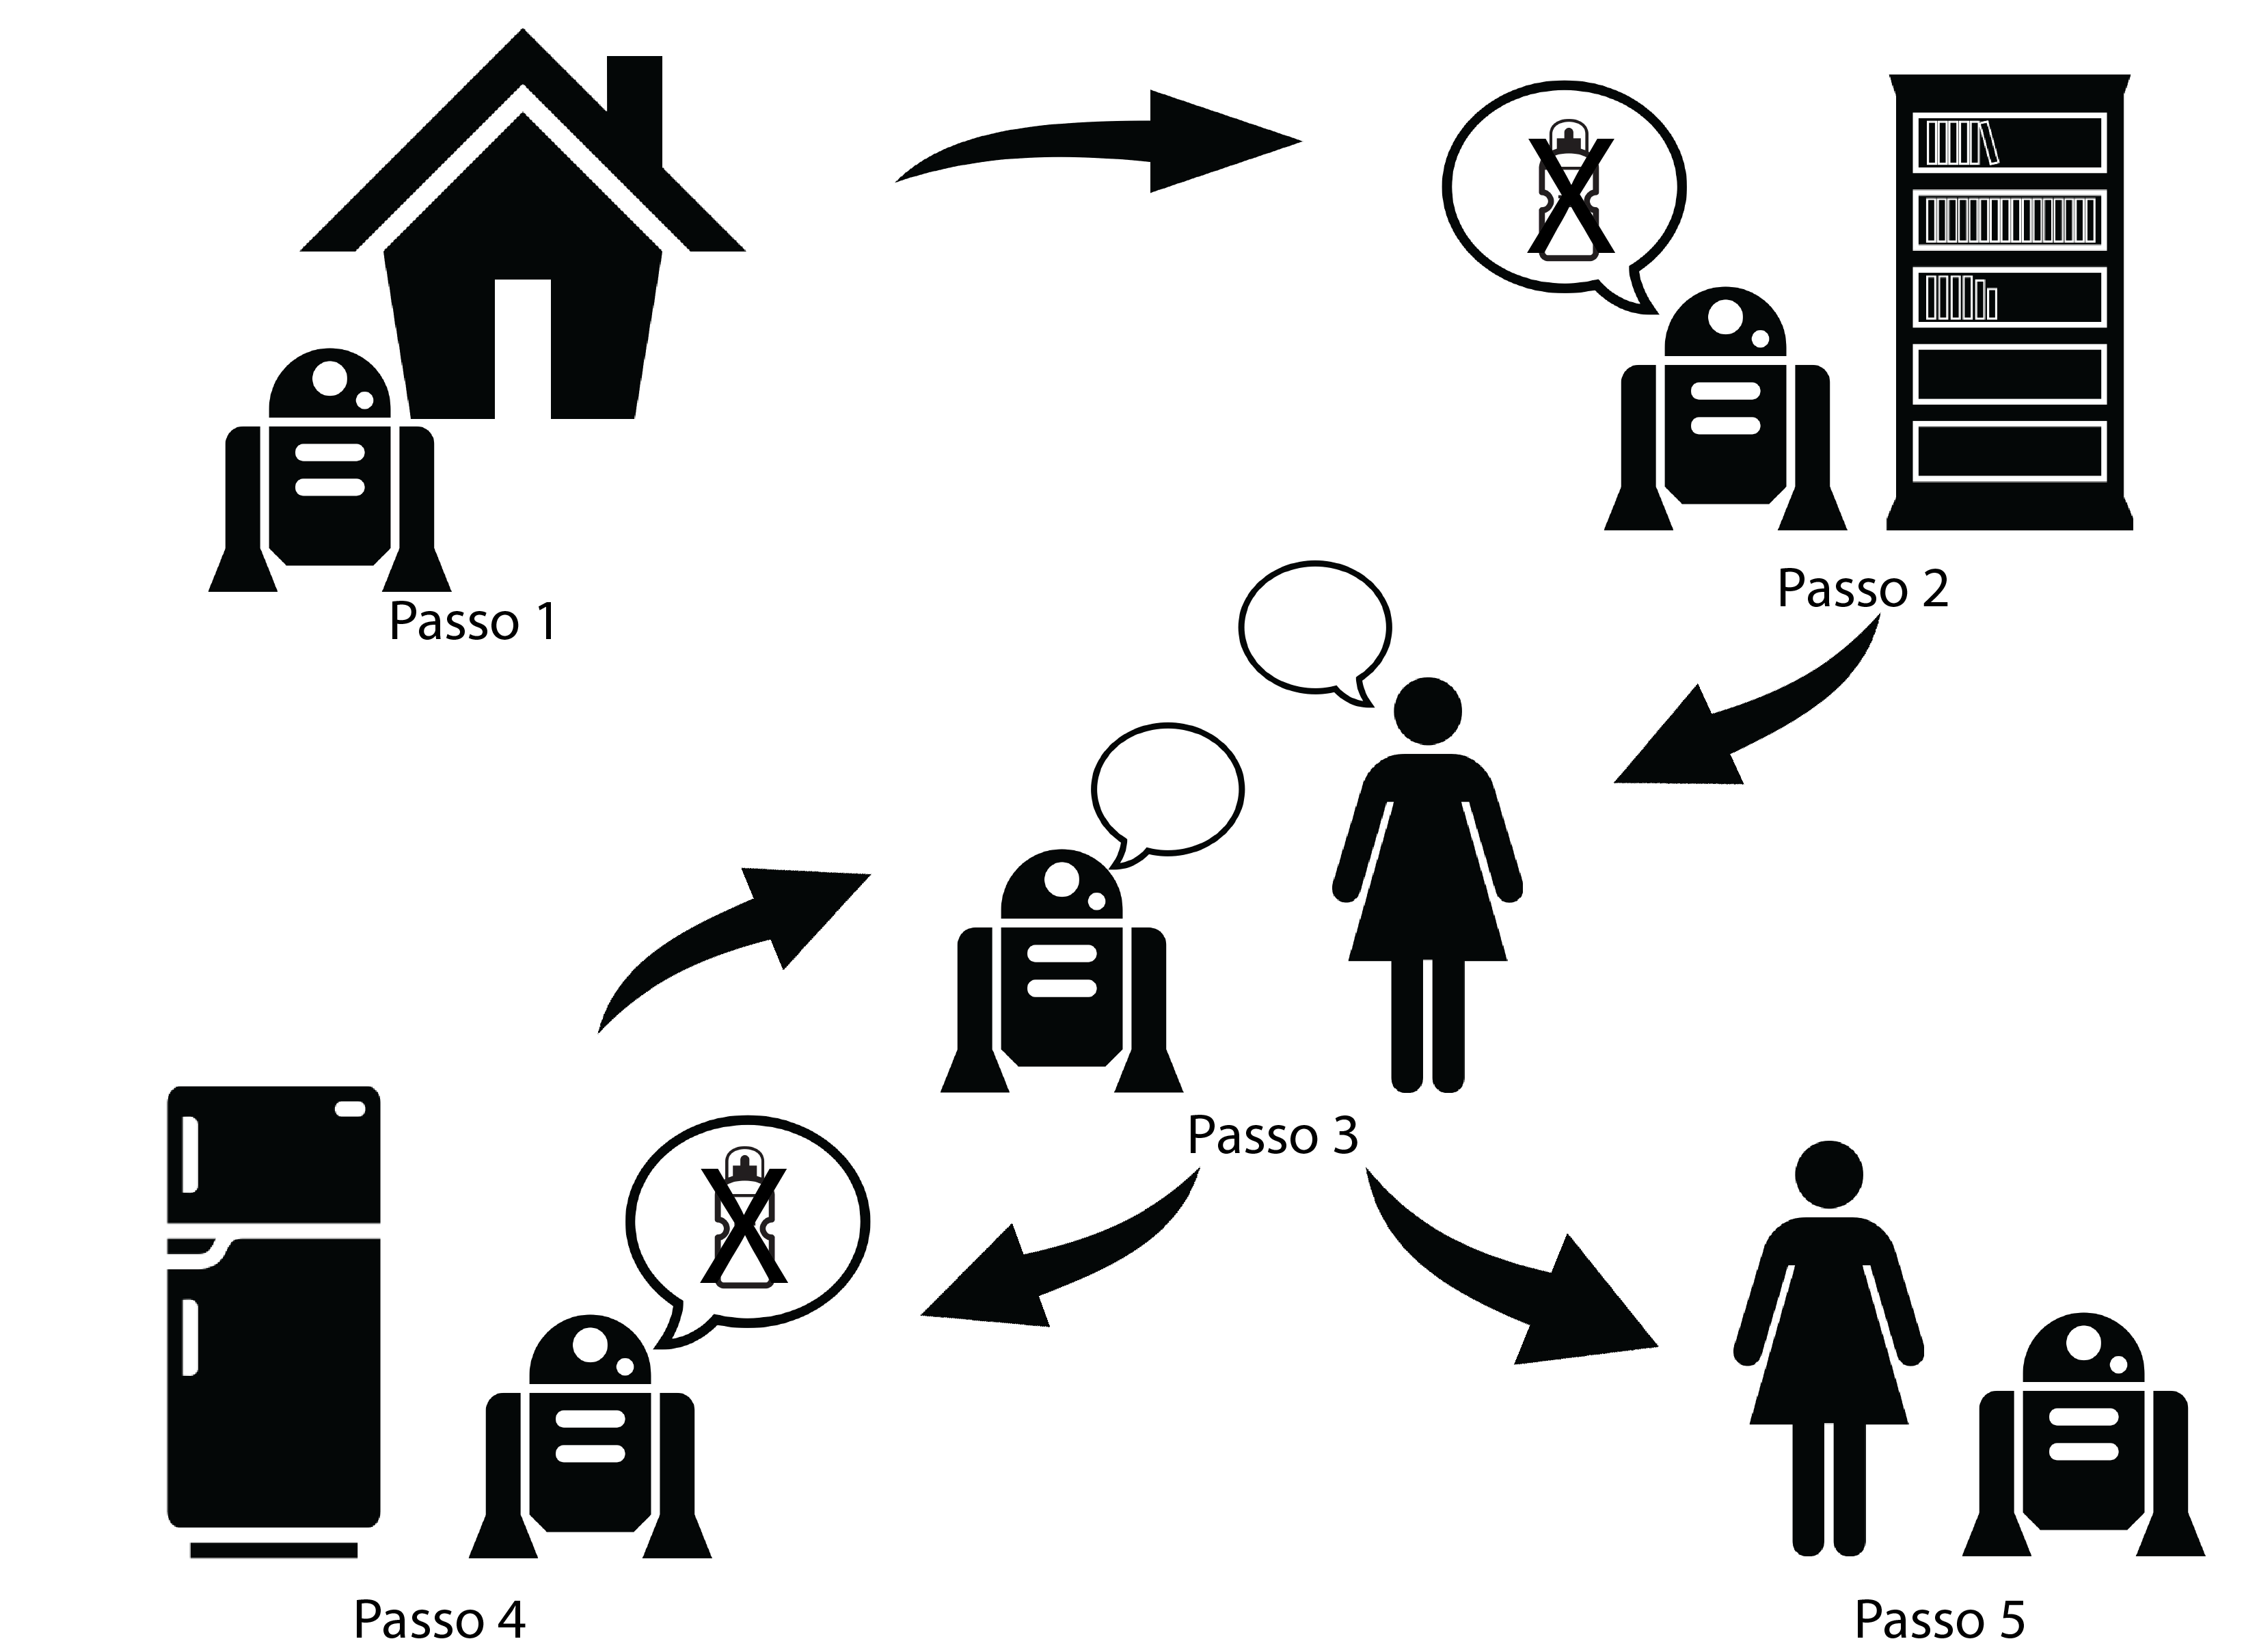
\includegraphics[width=\textwidth]{contexto-uso.png}
		\smallcaption{Fonte: o autor.}
		\label{fig:contextouso}
	\end{minipage}
\end{figure}

O cenário apresentado na figura~\ref{fig:contextouso} ilustra uma situação onde o robô entra em sua casa (passo 1) e vai até a estante onde ele deixou uma garrafa. A garrafa não está mais no local que ele deixou (passo 2), então ele vai até a pessoa que convive com ele no ambiente da casa. Ao interagir com a pessoa, o robô pergunta se ela viu a garrafa e recebe uma resposta negativa (passo 3). Na sequência, o robô procura pela garrafa em outro cômodo da casa, onde também não encontra (passo 4). O robô então retorna ao encontro da pessoa, e solicita a ajuda para procurar pela garrafa (passo 3). Como última etapa, a pessoa atende o pedido e ambos saem para procurar pela garrafa (passo 5), finalizando assim o cenário.

Através dessa ilustração pode-se definir o contexto de uso desta tese, onde o robô realiza a aproximação de pessoas que convivem com ele dentro de uma casa. Essa aproximação é realizada com o objetivo de solicitar ajuda ao humano para encontrar um objeto que foi deixado em algum lugar da casa. Com as variáveis identificadas e o contexto de uso da tese definidos, é necessário realizar a especificação do projeto, considerando fatores de engenharia de \emph{software} e fatores humanos já que existe interação humano-robô.

\section{Especificando o Projeto de IHR}
\label{sec:projetoihr}
Nos capítulos sobre IHR (capítulo~\ref{cap:ihr}) e teoria de proximidade (capítulo~\ref{cap:proxemics}) são apresentados diversos trabalhos com o estudos sobre interação entre humanos e robôs em diversas áreas, como saúde, lazer, entreterimento e social. Porém, ao analisar os projetos feitos nos trabalhos relacionados, não existe nenhuma definição sobre a especificação do projeto, como requisitos, perfis de usuários atentidos com o projeto, entre outros. O contexto de uso, em alguns casos, é utilizado pois, o projeto tem um foco em uma determinada tarefa. Contudo, projetos sem especificações são difícies de serem reproduzidos, um vez que os robôs utilizados são bem específicos. Além de serem específicos, os robôs utilizados são construídos, nos laboratórios das universidades e centros de pesquisas, em parte das pesquisas. As demais pesquisas utilizam robôs como: Softbank NAO~\footnote{https://www.ald.softbankrobotics.com/en/robots/nao} e PR2~\footnote{http://www.willowgarage.com/pages/pr2/overview}, que são produzidos por empresas especializadas fazendo com que o projeto fique restrito a sua capacidade determinada pela fábrica.

Em engenharia de \emph{software} são estudados vários métodos que auxiliam na especificação do projeto. Nesses métodos são encontrados a contemplação de alguns princípios que garantem a reprodução, manutenção e evolução do projeto ao longo tempo. Os princípios de engenharia de \emph{software} não são vistos como regras, mas como boas práticas para o desenvolvimento do projeto~\cite{wazlawick:2013}. As boas práticas aplicadas em sistemas computacionais, também podem ser aplicadas no desenvolvimento de projetos de robôs. Em seu trabalho \citeonline{wazlawick:2013} apresenta algumas boas práticas que a engenharia de \emph{software} provê aos projetos. A lista a seguir, descreve as boas práticas que contribuem para a evolução e formalização do projeto dessa tese.

\begin{itemize}
	\item \textbf{Decomposição}: é a criação de um \emph{software} ou produto a partir de um conjunto funcional de alto nível, os requesitos do projeto, onde esses são divididos em partes mais simples até chegar a um produto atômico, ou seja, partes de códigos. No robô, pode-se incluir também como os sensores e atuadores do projeto.
	\item \textbf{Padronização}: são importantes pois, através dos padrões conhecimentos adquiridos em projetos passados podem ser aplicados nos atuais evitando assim, que erros similares sejam cometidos.
	\item \textbf{Flexibilização}: auxilia na acomodação das mudanças de requisitos do projeto, No caso de robótica, nos cenários de atuação, diferentes contextos de uso, novos sensores e plataformas, entre outros.
	\item \textbf{Desenvolvimento Iterativo}: a cada momento novas necessidades são criadas e a partir da criação deve ser inseridas no projeto. Nas metodologias iterativas, cada ciclo de desenvolvimento é indepentende e deve entregar um produto operacional. Ao tratar de um projeto de interação humano-robô, pode-se dizer que o processo iterativo é longo e não necessariamente finito. Isso ocorre devido as novas necessidades dentre os diversos contexto de uso como hospitais, casas, hotéis, museus, resgate, shoppings, entre outros.
	\item \textbf{Arquiteturas baseadas em Componentes}: auxilia a lidar com complexidade do projeto e também o reuso e expansão. Cada sensor novo inserido no robô deve ser inserido junto a um novo módulo que captura as informações, consome os dados e entrega as informações para os componentes de tomada de decisão do robô, por exemplo.
\end{itemize}

Para garantir que as boas práticas sejam aplicadas no projeto, é necessário o uso de algumas ferramentas utilizadas dentro processo de criação de \emph{software}, aqui nessa tese utilizada na criação do projeto de interação humano-robô. O primeiro passo é definir as funcionalidades do sistema, que representam as ações que o robô pode executar. Depois é revisado os sensores e atuadores que contribuem com o objetivo voltado para cada funcionalidade. Por fim, o comportamento do sistema para cada funcionalidade, fechando assim a decrição dos requisitos do robô para o projeto.

\subsection{Definição das funcionalidades do robô}
\label{sec:funcionalidades}
Para criação das funcionalidades do robô utiliza-se as informações obtidas através do contexto de uso (vide seção~\ref{sec:contextouso}) e das variáveis de ações (vide seção~\ref{sec:acoes}). Cada variável é analisada e verifica como elas auxiliam no contexto de uso. A partir desse ponto, é criado um requisito para cada funcionalidade que contempla a variável. As variavéis de ações apresentadas na seção~\ref{sec:acoes} foram quase todas utilizadas para a criação das funcionalidades apresentadas nessa tese. A única variável não utilizada foi o volume da voz emitida pelo robô, pois os testes foram executados em ambiente público. A variação do volume nessa condição tornou-se inviável, pois ao diminuí-lo não era possível entender o que o robô dizia. Mais detalhes do ambiente de teste é apresentado na seção~\ref{sec:ambienteteste}.

A tabela~\ref{tab:funcionalidades} apresenta a relação de funcionalidades consideradas nessa tese e qual variável foi responsável pela funcionalidade.

\begin{table}[!ht]
	\caption{Funcionalidades do projeto de IHR.}
	\label{tab:funcionalidades}
	\centering
	\begin{tabular}{c | c | l}
        \hline
        Variável & ID & Funcionalidade \\
        \hline
		\multirow{3}{*}{Aproximação} & F01 & Reconhecer o ambiente \\
        \hhline{~--}
        & F02 & Controlar velocidade de navegação \\
        \hhline{~--}
        & F03 & Controlar proximidade da pessoa \\
        \hline
		\multirow{2}{*}{Manipulador} & F04 & Controlar gestos \\
        \hhline{~--}
        & F05 & Controlar força do manipulador \\
        \hline
		\multirow{2}{*}{Estilo de Voz} & F06 & Falar com diferentes níveis de ``educação'' \\
        \hhline{~--}
        & F07 & Identificar a fala da pessoa \\
        \hline
		\multirow{2}{*}{Expressão Facial} & F08 & Possuir diferentes estilos de face \\
		\hhline{~--}
		& F09 & Apresentar o estilo de face de acordo com a interação \\
		\hline
	\end{tabular}
	\smallcaption{Fonte: O autor.}
\end{table}

Cada uma das oito funcionalidades apresentadas na tabela~\ref{tab:funcionalidades} estão ligadas diretamente as interações previstas no contexto de uso. Para cada uma é necessário pelo menos um sensor para perceber os eventos externos ao robô e/ou um atuador para externar a funcionalidade ao objeto de interação. Os sensores e atuadores necessários são discutidos na seção~\ref{sec:sensoresatuadores}, a seguir.

\subsection{Listando sensores e atuadores necessários}
\label{sec:sensoresatuadores}
Com a lista de funcionalidades definidas, agora é necessário determinar quais são os sensores e atuadores do robô que serão capazes de atender cada uma das necessidades do projeto. Para a primeira funcionalidade F01 - Reconhecer o ambiente, o robô precisa de dois tipos de sensores, lasers e cameras de video. Esses sensores são capazes de determinar a distância entre um obstáculo e o robô, e também determinar o que ele enxerga no ambiente. Os atuadores envolvidos são os motores e servo-motores responsáveis pela locomoção do robô e movimento do manipulador.

Na funcionalidade F02 - Controlar Velocidade de Navegação, o robô necessita identificar quais são os obstáculos mais próximos para determinar qual velocidade ele por exercer na navegação. Para isso, é utilizado sensores lasers e atuação nos motores de movimentação do robô. A F02 está ligada a funcionalidade F03 - Controlar Proximidade da Pessoa. Na F03 o robô precisa de um sensor laser de movimento, como o Microsoft\textregistered\ Kinect\textregistered\ ou ASUS\textregistered\ Xtion\textregistered\, entre outros. Esses sensores conseguem determinar não só a profundidade entre obstáculos e o robô, mas também conseguem determinar o local da pessoa e quais partes do corpo dela estão mais próximas do robô. Dessa forma, é possível determinar a velocidade do motor para que o robô não atropele ou se aproxime de maneira ofensiva da pessoa.

As funcionalidades F04 - Controlar Gestos e F05 - Controlar Força do Manipulador, ligadas a variáveis manipulador, estão ligadas diretamente a atuação dos servo-motores presentes no manipulador. Para a F04 ainda é necessário o uso do Kinect\textregistered\ para verificar se não haverá colisão com a trajetória do manipulador. Já a força do manipulador correspondente a F05, é feito a leitura da corrente elétrica no servo-motor e caso haja um pico nela, o manipulador para o movimento e quando possível recua a posição inicial. Para a F06 - Falar com diferentes níveis de ``educação'', basta controlar via \emph{software} qual frase o robô emitirá através de seus alto-falantes. E na F07 - Identificar a fala da pessoa, é necessário um microfone direcional para auxiliar a eliminar o ruído do ambiente e capturar a voz da pessoa com que o robô interagirá.

Referente a expressão facial do robô, as funcionalidades F08 - Possuir diferentes estilos de face e F09 -
Apresentar o estilo de face de acordo com a interação, o robô necessita de uma tela que seja capaz de exibir suas expressões ao longo da sua interação. É importante atender essas funcionalidades dado o contexto da interação humano-robô ser social e entre agentes que convivem no mesmo ambiente. No caso desta tese, optou-se por um \emph{tablet} que fosse capaz de comportar um navegador \emph{web} que fosse capaz de interagir com o \emph{software} adotado no desenvolvimento do sistema.

A tabela~\ref{tab:sensoresatuadores} apresenta a síntese dos sensores e atuadores listados para atender as funcionalidades do projeto e portanto devem estar contidos no robô utilizado para interagir com o ser humano.

\begin{table}[!ht]
	\caption{Sensores e atuadores do projeto de IHR.}
	\label{tab:sensoresatuadores}
	\centering
	\begin{tabular}{c | l}
        \hline
        Categoria & Descrição \\
        \hline
		\multirow{4}{*}{Sensores} & Light Detection And Ranging (LIDAR) / Laser  \\
        \hhline{~-}
        & Sensor de movimento Microsoft\textregistered\ Kinect\textregistered \\
        \hhline{~-}
        & Camera de video \\
		\hhline{~-}
        & Microfone direcional do tipo shotgun (longo alcance) \\
        \hline
		\multirow{4}{*}{Atuadores} & \emph{Tablet} \\
        \hhline{~-}
        & Manipulador (Servo-motores) \\
		\hhline{~-}
        & Motores para locomoção \\
		\hhline{~-}
        & Alto-falantes \\
        \hline
	\end{tabular}
	\smallcaption{Fonte: O autor.}
\end{table}

Os detalhes de implementação de cada sensor e atuador listado na tabela~\ref{tab:sensoresatuadores}, é apresentado na seção~\ref{sec:robo} onde é discutido a preparação do robô para execução dos testes realizados. A seguir, na seção~\ref{sec:comportamentoesperado} é apresentado o comportamento que espera-se do robô ao atender as funcionalidades definidas.

\subsection{Comportamento esperado do robô}
\label{sec:comportamentoesperado}
Para cada funcionalidade, espera-se que o robô siga um padrão de comportamento. A apresentação desse padrão de comportamento será ilustrada vinculando os passos apresentados no contexto de uso, através da figura~\ref{fig:contextouso} e as funcionalidades apresentadas ao longo da seção~\ref{sec:funcionalidades}. No primeiro passo do contexto de uso, o robô deve ter em sua memória uma planta baixa do ambiente da casa que ele está inserido. A partir dessa planta é possível navegar até qualquer ponto desejado da casa. A navegação deve ser realizada de maneira onde o robô reconheça e desvie de obstáculos, e também controlando a velocidade para que seus movimentos sejam mais naturais a uma pessoa que vive na casa. Com esse comportamento, o robô atende as funcionalidades F01 e F02.

O passo dois no cenário do contexto de uso é verificar que, o objeto procurado não está no local esperado. Nesse momento o robô deve realizar uma comunicação visual e verbal para, caso haja uma pessoa em volta, perceba o que ocorreu. A comunicação visual pode ser feita através do manipulador e também do \emph{tablet} demonstra a expressão facial do robô. As funcionalidades F04, F06 e F08 estã contempladas através desse comportamento. Saindo do passo dois e avançando para o passo três, o robô atende as demais funcionalidades previstas. Ele busca pelo ser humano na casa, que ao encontrá-lo se expressa de maneira visual através do \emph{tablet}. Em seguida, o robô posiciona-se em frente a pessoa, identifica sua distância e transaciona com baixa velocidade até uma posição mais próxima da pessoa. Quando ele finalizou a aproximação, ele realiza um contato visual (gesto de olá) e sonoro (falando olá). Em sequência ele pergunta a pessoa se ela viu o objeto. A pessoa responde e eles segue para os demais passos. Os passos quatro e cinco são de comportamento similar aos passos anteriores.

A partir das definições e especificações feitas em relação ao projeto proposto por essa tese, deve-se na sequência realizar a preparação do robô e do ambiente para atender a todas questões debatidas ao longo da seção~\ref{sec:projetoihr}.

\section{Preparação do Robô}
\label{sec:robo}
O robô utilizado no desenvolvimento da tese é o PeopleBot~\footnote{PeopleBot - http://www.mobilerobots.com/researchRobots/PeopleBot.aspx} fabricado pela ActivMedia Robotics. Ele é um robô móvel com direção diferencial, ou seja, possui duas rodas motorizadas e uma roda castor que auxilia em seu equilíbrio. O projeto do PeopleBot tem foco em pesquisas e serviços que envolvem interação humano-robô. Com esse objetivo, ele foi desenvolvido com uma altura de 112 cm (centímetros). Além disso, o PeopleBot também possui uma garra pequena que tem sua movimentação apenas na direção vertical. A figura~\ref{fig:peoplebot} apresenta o robô PeopleBot.

\begin{figure}[ht!]
	\centering
	\begin{minipage}{\textwidth}
		\caption{Robô ActivMedia Robotics PeopleBot.}
		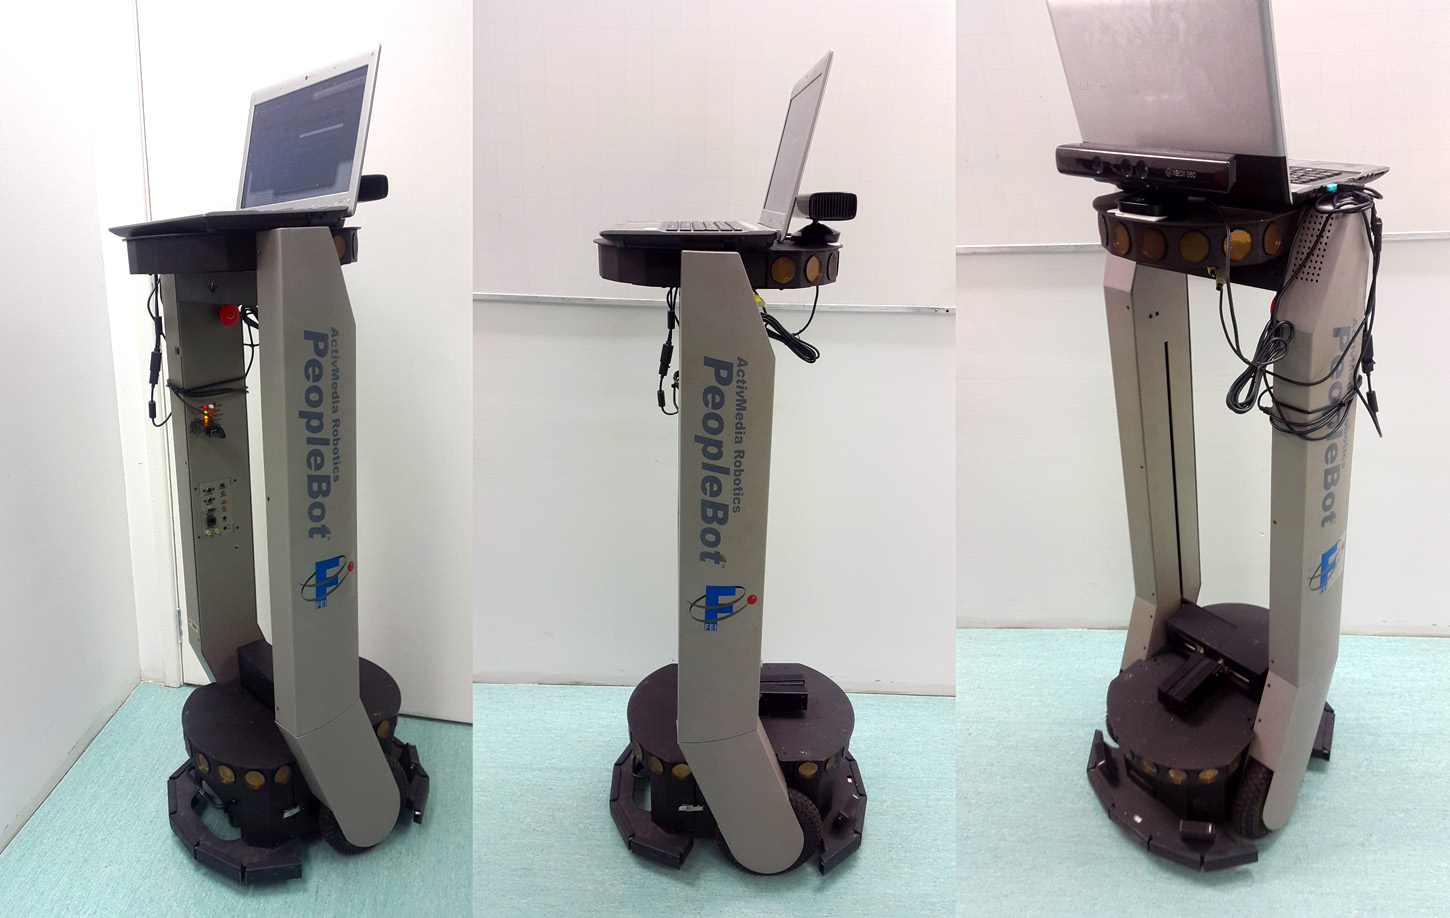
\includegraphics[width=\textwidth]{peoplebot.jpg}
		\smallcaption{Fonte: Autor.}
		\label{fig:peoplebot}
	\end{minipage}
\end{figure}

Como a garra do PeopleBot é curta e não permite muita destreza na manipulação de objetos e gestos, além de possuir poucos graus de liberdade, foi construído e adicionado um novo manipulador. O projeto do manipulador foi desenvolvido com o intuito de auxiliar a manipulação de objetos a uma certa distância e execução de gestos durante interações com pessoas. Esse novo manipulador é importante já que durante a interação social, seres humanos gesticulam para ilustrar a intenção e fala do que querem transmitir, por exemplo, acenar com as mãos ao falar olá. Esse tipo de comportamento aproxima naturalidade a interação humano-robô, podendo gerar um conforto a pessoa que interage. O projeto atende pesquisas com foco em prestação de serviços domésticos e cuidados pessoais, e foi construído de maneira que os movimentos sejam próximos do braço humano. O desenho que ilustra o manipulador desenvolvido é apresentado através da figura~\ref{fig:manipulador}.

\begin{figure}[ht!]
	\centering
	\begin{minipage}{0.6\textwidth}
		\caption{Projeto do Novo Manipulador do PeopleBot.}
		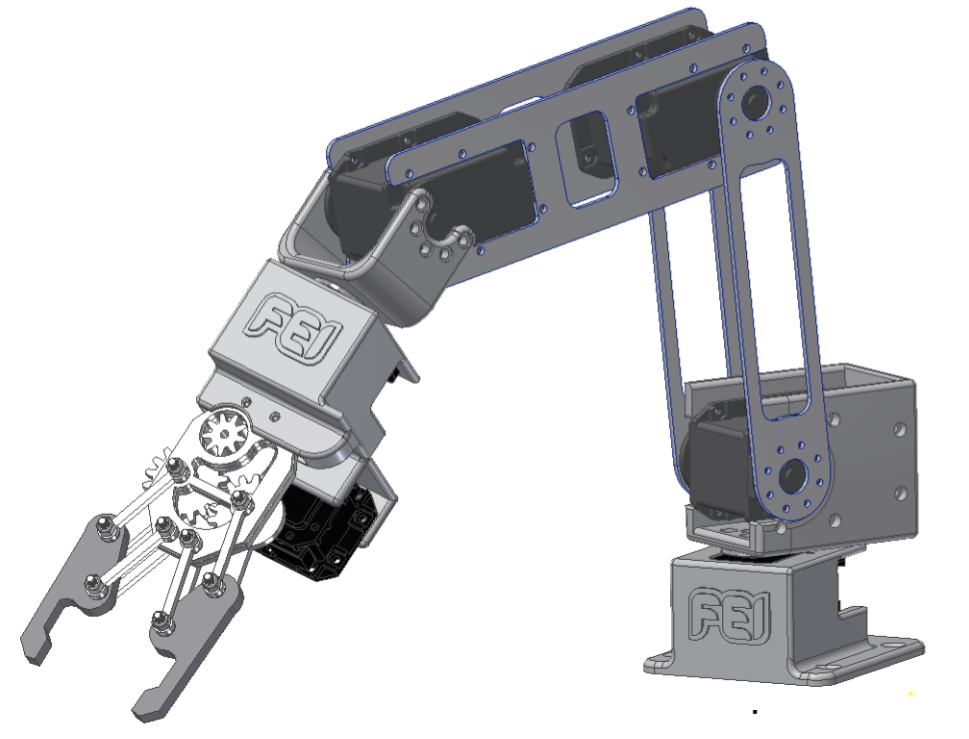
\includegraphics[width=\textwidth]{manipulador.png}
		\smallcaption{Fonte: \citeonline{gonbata:2016}.}
		\label{fig:manipulador}
	\end{minipage}
\end{figure}

Além do manipulador, também foi acoplado um \emph{tablet} para que seja possível atribuir face ao robô e consequentemente expressões faciais, deixando a interação mais amigável. O projeto da cabeça do robô é apresentado na figura~\ref{fig:judithhead}.

\begin{figure}[ht!]
	\centering
	\begin{minipage}{0.4\textwidth}
		\caption{Projeto da Cabeça para o PeopleBot.}
		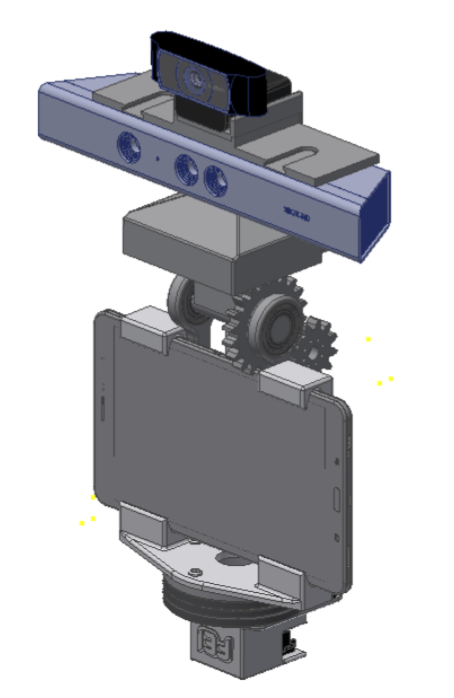
\includegraphics[width=\textwidth]{judith_head.png}
		\smallcaption{Fonte: \citeonline{gonbata:2016}.}
		\label{fig:judithhead}
	\end{minipage}
\end{figure}

O projeto da cabeça foi preparado para acomplar alguns alguns sensores como o Microsoft\textregistered\ Kinect\textregistered\ , o ASUS\textregistered\ Xtion\textregistered\ e webcams, para tarefas que envolvam nuvem de pontos de profundidade e visão computacional. Sensores como lasers e microfones também foram instalados para melhorar a captura de informações sobre o ambiente e interagir melhor com a pessoa. O sensor laser utilizado foi o Hokuyo URG-04LX-UG01 que possui um alcance de 5 metros, suficiente para navegação em um ambiente doméstico. O microfone, por se tratar de um ambiente com ruído e que a interação possuí diferentes distâncias para ocorrer, optou-se por um tipo \emph{shotgun} que tem o alcance de aproximadamente 2 metros. O modelo do microfone é o RODE Videomic Pro.

Durante os primeiros testes, a base do Peoplebot sofreu uma avaria e foi substituida por uma base da KUKA. É uma base com rodas omnidirecionais que proporcionam uma maior mobilidade de direções para o robô. A figura~\ref{fig:newjudith} apresenta a montagem final do robô para realização dos testes de interação na residência.

\begin{figure}[ht!]
	\centering
	\begin{minipage}{0.4\textwidth}
		\caption{Robô Judith na sua montagem final.}
		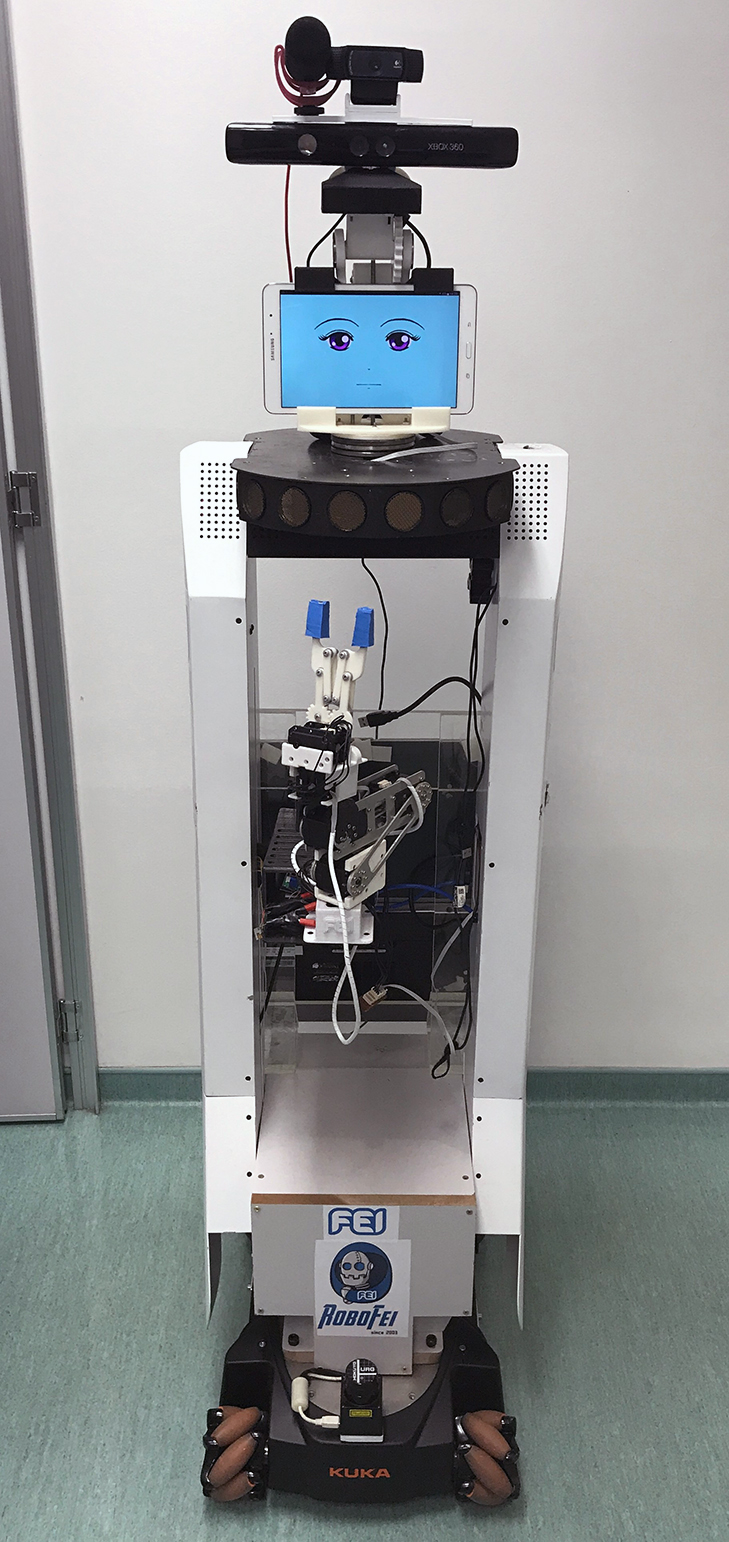
\includegraphics[width=\textwidth]{judith.jpg}
		\smallcaption{Fonte: Autor.}
		\label{fig:newjudith}
	\end{minipage}
\end{figure}

Além dos preparativos mecânicos para possibilitar a execução, de cada comportamento que atende as funcionalidades do projeto, também é necessário preparar os \emph{softwares} que irão compor a inteligência do robô. A arquitetura do robô e bibliotecas utilizadas para a composição do \emph{software} são apresentadas nas seções a seguir.

\subsection{Arquitetura do Software}
\label{sec:arquitetura}
A arquitetura construída para o software do robô foi feita em camadas. Existem 3 camadas principais, que definem a arquitetura do robô. A primeira camada contém os estados que compõem as máquinas de estados que auxiliam o robô nas tarefas a serem realizadas. Basicamente, ela conduz as ações e comandos que o robô tem como interface com o usuário durante a interação.

A segunda camada é responsável pelo processamento dos processos de \emph{subscribers} e \emph{publishers}, conforme o recomendado pelo \emph{Robot Operating System}~(ROS)~\footnote{http://www.ros.org/}. Eles fazem a interface entre sensores e atuadores, através de seus \emph{drivers}, e também com os algoritmos de visão computacional, de aprendizado de máquina e de planejamento. O processamento desses algoritmos, de sensores com grande volume de informação como o Kinect e serviços que auxiliam o controle do manipulador são encontrados na terceira camada.

Como toda a implementação do software foi feita com base no ROS, os pacotes foram construídos de maneira separada. Sendo assim, os códigos fontes ficaram agrupados de acordo com as habilidades necessárias para o robô realizar as tarefas e também referentes ao mesmo tipo de objetivo. Todo o código fonte criado para execução dos testes dessa tese, encontram-se disponível através do endereço \url{https://github.com/amasiero/approach_control}, na ferramente de controle de versão em código aberto, GitHub. O código foi testado com duas bases robóticas, o PeopleBot da Pioneer e o youBot da Kuka.

\subsection{Bibliotecas}
\label{sec:bibliotecas}
Para auxiliar no desenvolvimento da tese, algumas bibliotecas e softwares foram utilizados. O primeiro, conforme dito na seção~\ref{sec:arquitetura}, foi o ROS que é um \emph{framework} para desenvolvimento de software em robôs. Ele roda sobre o Ubuntu Linux, que no caso da tese foi utilizado a versão 14.04, com o ROS versão Indigo.

A biblioteca que gerencia a máquina de estados criada para execução das tarefas é o SMACH~\footnote{http://wiki.ros.org/smach}. Ele possibilita a criação e realiza o gerenciamento dos estados durante a execução das ações do robô. Para reconhecimento de voz a biblioteca utilizada foi o Dragonfly Speech Recognition~\footnote{https://pypi.python.org/pypi/dragonfly/0.6.5}. Bibliotecas como o OpenCV~\footnote{http://opencv.org/}, PyOpenni~\footnote{https://github.com/jmendeth/PyOpenNI} e MoveIt!~\footnote{http://moveit.ros.org/} foram utilizados para percepção e interação com o ambiente e também com o usuário.

Todos os pacotes desenvolvidos utilizaram a linguagem de programação Python, que possibilitou diversas facilidades na implementação dos códigos e integração das camadas dos pacotes no ROS. Para criação e teste da rede bayesiana proposta utilizou-se o \emph{framework} SamIam~\footnote{http://reasoning.cs.ucla.edu/samiam/}, que realiza os cálculos de todas as probabilidades de uma consulta a rede de maneira objetiva.

\section{Preparando o Ambiente de Teste}
\label{sec:ambienteteste}
O teste é realizado em um ambiente que simula uma residência, conforme apresentado na figura~\ref{fig:cenario}. No ambiente, o robô irá navegar de maneira autonoma a procura de uma garrafa que ele deixou no armário. Como ele não encontra a garrafa, o robô sai a procura de uma pessoa que esteja na casa para ajuda-lo. Ele irá interagir com a pessoa, e poderá solicitar que a pessoa o siga para algum lugar do cenário, à procura de sua garrafa. Tudo essas tarefas estão de acordo com as necessidades do projeto e também do seu contexto de uso, conforme apresentado nas seções anteriores deste capítulo.

\begin{figure}[ht!]
	\centering
	\begin{minipage}{\textwidth}
		\caption{Cenário para teste de interação com o robô.}
		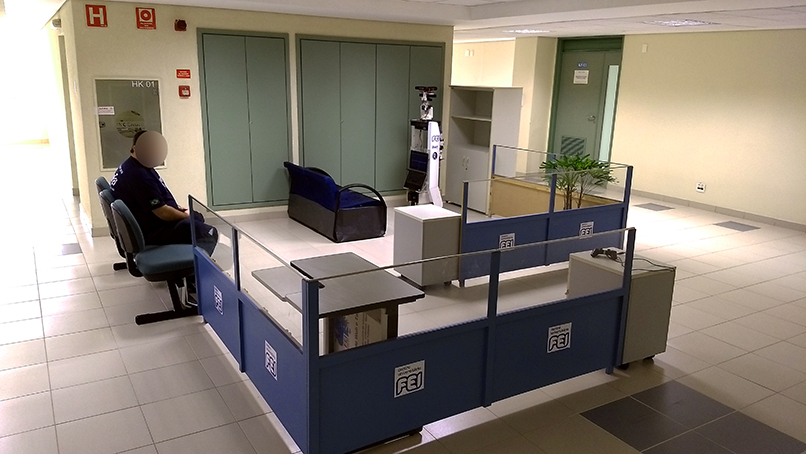
\includegraphics[width=\textwidth]{cenario.jpg}
		\smallcaption{Fonte: Autor.}
		\label{fig:cenario}
	\end{minipage}
\end{figure}

\subsection{Objetivo}

Verificar a compreensão e conforto da pessoa ao observar e interagir com o robô no ambiente doméstico, afim identificar experiências positivas e negativas por parte do usuário.

\subsection{Configuração para o Teste}

Para o teste são consideradas algumas possibilidades de posicionamento da pessoa e robô para interagirem.

\begin{itemize}
	\item Pessoa parada em pé e o robô inicia a interação próximo do usuário.
	\item Pessoa parada em pé e o robô inicia a interação distante do usuário.
	\item Pessoa parada sentada e o robô inicia a interação próximo do usuário.
	\item Pessoa parada sentada e o robô inicia a interação distante do usuário.
\end{itemize}

O objetivo das configurações é a aleatoriedade do posicionamento entre robô e pessoa, considerando cenários doméstico onde o convívio é comum. Assim, é possível medir a experiência do usuário em diversas situações de convivência.

\subsection{Tarefa}

Esse teste ocorre em um ambiente controlado, porém o trânsito de outros indíviduos pelo cenário acontece com frequência significativa. O passo a passo da tarefa é descrito na lista a seguir:

\begin{enumerate}
	\item \textbf{Início}: O robô é posicionado no cenário de maneira que esteja em um local em torno da residência simulada.
	\item \textbf{Busca pelo objeto}: O robô segue até uma mesa, ou armário, onde supostamente deixou sua garrafa.
	\item \textbf{Interação com a pessoa}: O robô se aproxima do usuário e questiona se ele viu a garrafa.
	\item \textbf{Nova busca pelo objeto}: O robô segue a um novo ponto em busca da garrafa, que novamente não está no local.
	\item \textbf{Retorno ao usuário}: O robô retorna ao local onde o usuário se encontra e, em uma distância maior ou menor de proximidade (aleatória), solicita que o usuário o acompanhe.
	\item \textbf{Fim}: Será considerado o fim da tarefa, quando o robô alcançar um ponto ao redor do cenário e informar o fim do teste ao participante.
\end{enumerate}

As tarefas são definidas com base no contexto de uso ilustrado através da figura~\ref{fig:contextouso}. Nesse ponto, o projeto está especificado, os equipamentos e ambiente prontos para realizar a interação humano-robô. Como é um experimento que envolve testes com ser humano, é importante enviar o projeto para apreciação do comitê de ética através da ferramenta Plataforma Brasil~\footnote{http://plataformabrasil.saude.gov.br/login.jsf}. Esse projeto tem a aprovação do comitê de ética, através do número de processo CAAE: 70057117.0.0000.5508.

\section{Construção do Questionário Pré Teste}
\label{sec:questionariopreteste}
Para apoiar o processo de obtenção das informações e construção dos perfis dos usuários, são utilizados dois questionários. O primeiro, aplicado no momento anterior ao experimento de interação, tem como objetivo mapear as informações referentes às características físicas que tem a possibilidade do robô utilizar sensores para reconhecê-las, adesão a tecnologia, contatos prévios com robôs, questões culturais onde o usuário declara quais locais ele possui mais afinidade e quais ele já teve o privilégio de visitar, além da expectativa de possuir um robô em casa ou no trabalho. As questões são apresentadas na tabela~\ref{tab:questoespreteste}, onde a coluna construção contém os grupos de informações que conferem com a parte do perfil que elas auxiliam a preencher conforme apresentado por \citeonline{barbosa:2010} e \citeonline{baxter:2015}. Todas as questões a seguir fazem para do questionário pré-experimento.

\begin{longtable}{ m{7 cm} | m{4cm} | m{4cm} }
	\caption{Questões aplicadas no questionário pré teste }
	\label{tab:questoespreteste} \\	\hline
	Pergunta & Opções & Construção \\ \hline
	Informe seu nome completo & Texto Aberto & Identificação \\ \hline
	e-mail para contato & Texto Aberto & Contato Usuário \\ \hline
	Informe o número do seu celular & Texto Aberto & Contato Usuário \\ \hline
	Testes poderão ocorrer usando o Robô no Centro Universitário FEI. Você gostaria de realizar o teste com o robô físico? & Sim; Não & Contato Usuário \\ \hline
	Qual a sua idade? (em anos) & Númerico & Demográfico \\ \hline
	Qual a sua altura? (em metros) & Númerico & Demográfico \\ \hline
	Informa seu gênero & Feminino; Masculino; Prefiro não dizer & Demográfico \\ \hline
	Na maior parte do tempo, você se considera uma pessoa com feição: & Sorridente; Normal; Séria/Fechada & Social \\ \hline
	Você se considera uma pessoa sociável? & Sim; Não & Social \\ \hline
	Você utiliza óculos de grau? (Obs: Pessoas com lente de contato, por favor, repondam não. A intenção é identificar a armação.) & Sim; Não & Físico \\ \hline
	Você possui cabelo comprido? & Sim; Não & Físico \\ \hline
	Qual etnia você se considera? & Amarela; Branca; Indígena; Parda; Preta; Não declarada & Etnográfico \\ \hline
	Qual(is) dispositivo(s) tecnológico(s) você mais utiliza (marque 1 ou mais opções): & Celular; Computador (de mesa ou notebook); Tablet; Smart TV; Relógio Smart; MP3 Player; Câmera Fotográfica Digital; Leitor de e-Book; outros & Experiência com Tecnologias \\ \hline
	Qual(is) dispositivo(s) tecnológico(s) você nunca utilizou (marque 1 ou mais opções): & Celular; Computador (de mesa ou notebook); Tablet; Smart TV; Relógio Smart; MP3 Player; Câmera Fotográfica Digital; Leitor de e-Book; Já utilizei todas & Experiência com Tecnologias \\ \hline
	Você possui conta em banco digital (ex: Original, Neon, etc.) ? & Sim; Não & Atitudes e Valores \\ \hline
	Você possui cartão de crédito digital (ex: Nubank, Digio, etc.) ? & Sim, Não & Atitudes e Valores \\ \hline
	Qual o principal meio de pagamento de suas contas? & Celular; Computador; Tablet; Autoatendimento; Caixa Físico & Atitudes e Valores \\ \hline
	Você utiliza redes sociais? & Sim; Não & Experiência com Tecnologias \\ \hline
	Quais as redes sociais que você mais utiliza (marque 1 ou mais opções): (Se sim, para a resposta anterior) & Facebook, Instagram, Twitter, Google\+, Snapchat, outras& Experiência com Tecnologias \\ \hline
	Qual foi o local de nascimento? (Informe da seguinte maneira: Cidade; Estado; País) & Texto Aberto & Cultural \\ \hline
	Em qual local, você viveu por mais tempo durante sua infância e adolescência? (Informe da seguinte maneira: Cidade; Estado; País) & Texto Aberto & Cultural \\ \hline
	Qual o seu atual local de moradia? (Informe da seguinte maneira: Cidade; Estado; País) & Texto Aberto & Cultural \\ \hline
	Qual o país que você melhor se identifica com a cultura? (Considere também a opção do seu país de nascimento.) & Texto Aberto & Cultural \\ \hline
	Qual a cidade, na sua opinião, que melhor representa a cultura que você se identifica (resposta não dependente da questão acima)? & Texto Aberto & Cultural \\ \hline
	Você visitou outros países, além do Brasil? & Sim; Não & Cultural \\ \hline
	Quais países você já visitou? (Responda separando os países por ponto e vírgula, ex: França; Estados Unidos; Itália; Japão;) & Texto Aberto & Cultural \\ \hline
	Aproximadamente, quantas cidades na região nordeste do Brasil você visitou? & Numérico & Cultural \\ \hline
	Aproximadamente, quantas cidades na região norte do Brasil você visitou? & Numérico & Cultural \\ \hline
	Aproximadamente, quantas cidades na região centro-oeste do Brasil você visitou? & Numérico & Cultural \\ \hline
	Aproximadamente, quantas cidades na região sudeste do Brasil você visitou? & Numérico & Cultural \\ \hline
	Aproximadamente, quantas cidades na região sul do Brasil você visitou? & Numérico & Cultural \\ \hline
	Em algum momento de sua vida, você teve contato com robôs? & Sim; Não & Experiência com Produto \\ \hline
	Se sim para a questão anterior, quais tipos de robôs você teve contato (marque 1 ou mais opções): Opções de resposta: Parecido com animais, Parecido com pessoas, Robôs de linha de produção/fábrica, Robôs Móveis (que contém rodas), outros  & Experiência com Produto \\ \hline
	O que você espera do comportamento do Robô ao tê-lo em sua casa? & Texto Aberto & Experiência com Produto \\ \hline
	O que você espera do comportamento do Robô ao tê-lo em seu trabalho? & Texto Aberto & Experiência com Produto \\ \hline
	Dadas as questões anteriores, gostaria de fazer mais algum comentário sobre você? & Texto Aberto & Comentários Aberto \\ \hline
	\smallcaption{Fonte: O autor.}
\end{longtable}

A partir das informações coletadas com as questões apresentadas na tabela~\ref{tab:questoespreteste}, é possível determinar o perfil de cultura declarado pelo usuário, informações etnográficas que irão auxiliar na identificação da Persona. Expectativas sobre a interação com robôs em ambientes domésticos e profissionais, também são adquiridas. Essas informações auxiliam a determinar o ponto de partida para a análise e criação das personas discutidas no capítulo~\ref{cap:proposta}.

\section{Interação entre o Usuário e o Robô}
\label{sec:experimentointeracao}
Nesse ponto o usuário é convidado a interagir com o robô. O especialista posiciona o usuário no ambiente de teste, onde ele pode ficar sentado ou em pé. Câmeras são posicionada de maneira que o possam capturar as reações que o usuário terá durante toda a interação com o robô. O especialista explica todos os procedimentos do experimento e da o sinal para que o robô inicie o teste. O sinal ocorre através de um comando de voz para o robô. Durante todo o experimento o usuário é incentivado a falar em voz alta o que está passando pela sua cabeça. Com as informações faladas e observações visuais, que são feitas pelo próprio especialista, são gerados pontos de atenção para melhoria e até pontos de sucesso no projeto. Ao final, o usuário é encaminhado para preencher o questionário pós teste, apresentado em detalhes na seção~\ref{sec:questionarioposteste}.

É importante delimitar os usuários que farão o testes de maneira criteriosa. Os perfis dos selecionados podem levar a diferentes resultados na interação. Os usuários selecionados para realizar o teste, são denominados de sujeito de teste. Nessa tese o seguinte perfil foi utilizado: pessoas que possuem idades diversificadas com variedade de 18 a 70 anos. Alguns candidatos ao teste possuem medo declarado de robôs e neste caso o especialista ficará acompanhando o teste com uma maior proximidade para evitar problemas com o robô e principalmente com a pessoa.

São evitados a repetição de configuração entre os candidatos, para que não seja levantado nenhum conhecimento a priori sobre o comportamento do robô.

\section{Construção do Questionário Pós Teste}
\label{sec:questionarioposteste}
O questionário pós teste mantém o foco na interação do usuário que ocorreu durante o experimento e quais pontos do robô mais agradaram em sua opinião. Além disso, um detalhe sobre a posição do usuário durante o experimento (sentado ou em pé) é coletada, pois esta informação pode influenciar na interação com o robô. As questões apresentas na tabela~\ref{tab:questoesposteste}, a seguir, compõe o questionário pós-teste.

\begin{longtable}{ m{7 cm} | m{4cm} | m{4cm} }
	\caption{Questões aplicadas no questionário pós teste }
	\label{tab:questoesposteste} \\	\hline
	Pergunta & Opções & Construção \\ \hline
	Informe o número de amostra (Identificador dos documentos referentes ao comitê de ética) & Numérico & Identificação \\ \hline
	Você se sentiu confortável durante a aproximação do robô? & Escala Likert de 10 pontos & Satisfação \\ \hline
	Você se sentiu com medo em algum momento durante a aproximação do robô? & Escala Likert de 10 pontos & Satisfação \\ \hline
	Você estava \_\_\_\_\_\_\_\_\_ durante a aproximação do robô. & Sentado; em Pé & Uso \\ \hline
	Você voltaria a interagir com esse robô novamente? & Sim; Não & Satisfação \\ \hline
	Justifica a resposta anterior & Texto Aberto & Satisfação \\ \hline
	O que você mais gostou no robô? & Texto Aberto & Satisfação \\ \hline
	O que você menos gostou no robô? & Texto Aberto & Satisfação \\ \hline
	Depois dessa experiência, você interagiria com outros robôs? & Sim; Não & Satisfação \\ \hline
	Você estaria confortável com um robô convivendo em sua casa? & Sim; Não & Satisfação \\ \hline
	Justifique a resposta anterior. & Texto Aberto & Satisfação \\ \hline
	Em algum momento da interação, você se sentiu desconfortável com o comportamento do robô? & Sim; Não & Uso \\ \hline
	Descreva o desconforto em caso de sim, na resposta anterior. & Texto Aberto & Uso \\ \hline
	Você alteraria algum comportamento apresentado pelo robô durante o teste? Qual? & Texto Aberto & Uso \\ \hline
	Observações e comentários: & Texto Aberto & Comentários Aberto \\ \hline
	\smallcaption{Fonte: O autor.}
\end{longtable}

Esse questionário tem o principal objetivo de coletar as informações que o usuário declarou não haver gostado na interação. As declarações ajudam a compreender o que deixou ele desconfortável e/ou com medo facilitando na hora de confortar com as observações do especialista realizadas durante a interação.

\section{Observando o Teste}
\label{sec:observacoesteste}
Durante a execução do experimento, o especialista deve fazer anotações que contribuam com o futuro do projeto. Esse é um processo similar ao teste com usuário realizado em projetos de interação humano-computador. No processo de informação são feitas anotações sobre o usuário, que ele não comunica através dos questionários. Outro ponto importante da etapa de observação é a entrevista realizada após o teste, onde o especialista realiza perguntas abertas para que o usuário fique a vontade em dizer mais sobre o produto e como ele se sentiu em determinadas ocorrências.

Essas informações são utilizadas para agregar mais conhecimento durante o processo de análise dos resultados. Os dados da primeira rodada de testes realizados no desenvolvimento dessa tese, servem de insumo para a construção de um classificador de perfil de usuário, apresentado no capítulo~\ref{cap:proposta}.

\section{Processo de Análise das Observações e Respostas}
\label{sec:analise}
As informações coletadas através dos questionários e observações, são utilizadas no processo de definição das probabilidades referentes as tabelas condicionais das variáveis aleatórias, que compõem a rede bayesiana. Além disso, auxiliam na contextualização da descrição sobre a Persona que representará os usuários. O processo de análise é feito através da classificação de comportamentos e declarações realizados durante o teste. Essa classificação tem base na ocorrência das informações durante as observações entre os diversos testes que ocorreram. O resultado dessa análise é feito em mais detalhes ao longo do capítulo~\ref{cap:proposta}, apresentado a seguir.
